% This is LLNCS.DEM the demonstration file of
% the LaTeX macro package from Springer-Verlag
% for Lecture Notes in Computer Science,
% version 2.4 for LaTeX2e as of 16. April 2010
%
\documentclass{llncs}
%
\usepackage{makeidx}  % allows for indexgeneration
% For figures
\usepackage{graphicx} % more modern
%\usepackage{epsfig} % less modern
\usepackage{subfigure} 
\usepackage{color}
%\usepackage{subfig}%[caption=false,font=footnotesize]

% For citations
\usepackage{natbib}

% For algorithms
\usepackage{algorithm}
\usepackage{algorithmic}

% As of 2011, we use the hyperref package to produce hyperlinks in the
% resulting PDF.  If this breaks your system, please commend out the
% following usepackage line and replace \usepackage{icml2012} with
% \usepackage[nohyperref]{icml2012} above.
\usepackage{hyperref}

% Packages hyperref and algorithmic misbehave sometimes.  We can fix
% this with the following command.
\newcommand{\theHalgorithm}{\arabic{algorithm}}

%-------------------------------------------------------------
%                      Own Commands
%-------------------------------------------------------------
\usepackage{amsmath}
\newcommand{\cbn}{\textsc{Cbn}}
\newcommand{\bn}{\textsc{Bn}}
\newcommand{\huang}[1]{\textcolor{blue}{#1}}
\newcommand{\mycomment}[1]{\textcolor{red}{( ...#1 )}}
\renewcommand{\algorithmiccomment}[1]{/* #1 */}
\def\ci{\perp\!\!\!\perp}
\def\dep{\perp\!\!\!\perp\!\!\!\!\!\!\!/\,\,\,\,}
% Theorem & Co environments and counters
%\newtheorem{theorem}{Theorem}[section]
%\newtheorem{lemma}[theorem]{Lemma}
%\newtheorem{corollary}[theorem]{Corollary}
%\newtheorem{remark}[theorem]{Remark}
%\newtheorem{definition}[theorem]{Definition}
\newtheorem{equat}[theorem]{Equation}
%\newtheorem{example}[theorem]{Example}
%-------------------------------------------------------------

\begin{document}
%
\frontmatter          % for the preliminaries
%
%\pagestyle{headings}  % switches on printing of running heads
%\addtocmark{Hamiltonian Mechanics} % additional mark in the TOC
%%
%\tableofcontents
%
\mainmatter              % start of the contributions
%
\title{ Communication-efficient Learning from Multiple Experts}
%
%\titlerunning{Hamiltonian Mechanics}  % abbreviated title (for running head)
%                                     also used for the TOC unless
%                                     \toctitle is used
%
\author{Bojan  Kolosnjaji\inst{1} \and Huang Xiao\inst{2} 
	\and Claudia Eckert\inst{1}\inst{2} }
%Jeffrey Dean \and David Grove \and Craig Chambers \and Kim~B.~Bruce \and
%Elsa Bertino}
%
\authorrunning{Bojan Kolosnjaji et al.} % abbreviated author list (for running head)
%
%%%% list of authors for the TOC (use if author list has to be modified)
%\tocauthor{Ivar Ekeland, Roger Temam, Jeffrey Dean, David Grove,
%Craig Chambers, Kim B. Bruce, and Elisa Bertino}
%
\institute{Technical University of Munich, Fraunhofer AISEC\\
\email{kolosnjaji@sec.in.tum.de, huang.xiao@aisec.fraunhofer.de, eckert@sec.in.tum.de}
%\\ WWW home page:
%\texttt{https://www.aisec.fraunhofer.de/}
%\and
%Universit\'{e} de Paris-Sud,
%Laboratoire d'Analyse Num\'{e}rique, B\^{a}timent 425,\\
%F-91405 Orsay Cedex, France
}

\maketitle              % typeset the title of the contribution

\begin{abstract}
Learning from multiple sources of labeled data can increase the confidence of a machine learning system if the expertise of different labelers can be assembled efficiently. However, using a large amount of labelers in the test time can be expensive in the long run. For instance, in crowdsourcing, we have to pay each labeler in order to get the annotations. In Internet-of-Things, obtaining data from multiple sensors for
direct fusion incurs high communication overhead. 

In this paper, we propose a method for training a classification system from data labeled by multiple client annotators, where only a small subset of annotators are optimally chosen to reduce communication effort. 
We define an iterative optimization procedure where the sparsity of a client weight vector is enforced while reducing the overall classification error. Using a set of experiments, we show that our approach can pertain the classification performance as on the complete set of labelers while reducing the communication effort by over 70\% on several different tasks.

%submit  abstract until 13.04

\keywords{machine learning, communication-efficiency, crowdsourcing, Internet-of-Things}
\end{abstract}
%

\section{Introduction}
Machine Learning systems depend on our ability to gather a large set of data. In a large number of scenarios, we gather labeled data from multiple separate sources with varying reliability and join this data into one machine learning model. Furthermore, many times we are limited in how many data sources we are allowed to use, because of budget constraints, limited processing power or insufficient communication bandwidth.

First important fitting scenario is crowdsourcing. When using crowdsourcing systems such as Amazon Mechanical Turk, we can gather labelled data from multiple annotators. After gathering this training data, we need to join the labelling decisions and train one machine learning system while leveraging all of the annotations. Relying on a concept of \textit{wisdom of crowds}, we can assume that if we gather data from a sufficient number of people, on average most of them will give correct labelling decision. However, gathering data from a large amount of annotators can be expensive, as workers on Amazon Mechanical Turk require payment for their work. There fore we would benefit from a procedure of prior determination of the expertise of the annotators. In this case, the joining process can be optimized by estimating the expertise of the annotators, selecting the most reliable ones and determining weights of their decisions. 

Moreover, in a rising area of \textit{Internet of Things} (IoT)we can have similar problems. In IoT systems, a large number of sensors provide information about the environment. Communication among multiple sensors can be costly in terms of processing power. Furthermore, this communication can be done among sensors that are limited with power consumption constraints.

There are multiple papers that deal with estimating the expertise of labelers when using \textit{wisdom of crowds}. For example, Welinder et al. \cite{welinder2010multidimensional} determine groups of annotators with similar expertise, and find particular phenomena such as "schools of thought" and specialist experts in certain types of image labeling tasks. Tian and Zhu~\cite{tian2012learning} investigate the annotator behavior in executing more complex labeling tasks, such as answering if an image is beautiful or if it contains a car. Zhang et al.~\cite{zhang2013learning} propose a method to filter out novice labelers. However, their method is specific to Gaussian Mixture Model. Rodrigues et al.~\cite{rodrigues2014gaussian} determine a similar procedure specific to Gaussian Processes. Bi et al.~\cite{bi2014learning}argue that the factors that determine the annotators' labeling performance, apart from the expertise, can also be the worker's dedication to the task, his/her default labeling judgement and sample difficulty. However, they do not go further in determining the optimal subset of annotators. On the other hand, Li and Liu~\cite{li_liu_2015} propose a combinatiorial procedure to find this optimal subset. However, such combinatorial procedures are very resource-intensive, especially for a large initial set of annotators.

On the other hand, there are are also multiple more theoretical frameworks. For example, Wang et al.~\cite{wang2015efficient} propose a selection of sensors based on Directed Acyclic Graphs (DAGs) in resource-constrained scenarios. However, they do not deal with annotating data, so their ideas does not completely fit to our problem. 

We design a methodology that both selects an optimal set of annotators from a set of training data and automatically determines the weights of the selected annotators. By forcing sparsity on our annotator weight vector, we get an accurate classification system that works well even with annotations from a small set of highly competent annotators.

In summary, we make the following contributions:
\begin{itemize}
\item We propose a methodology for selecting an optimal subset of workers in a classification system with multiple labelers
\item We create a procedure for selecting and determine weights of labelers independent of type machine learning methods selected for modeling the annotating process
\item Using a set of experiments with real and synthetic data, we show that we can obtain accurate classification system with a learned annotator subset.
\end{itemize}  


\section{Methodology}

Our methodology is based on the scenario drawn on the \autoref{fig:scheme}. This scheme shows a common situation when a server gets labells from multiple annotators. 

\begin{figure}
  \caption{Label aggregation scheme}
  \centering
    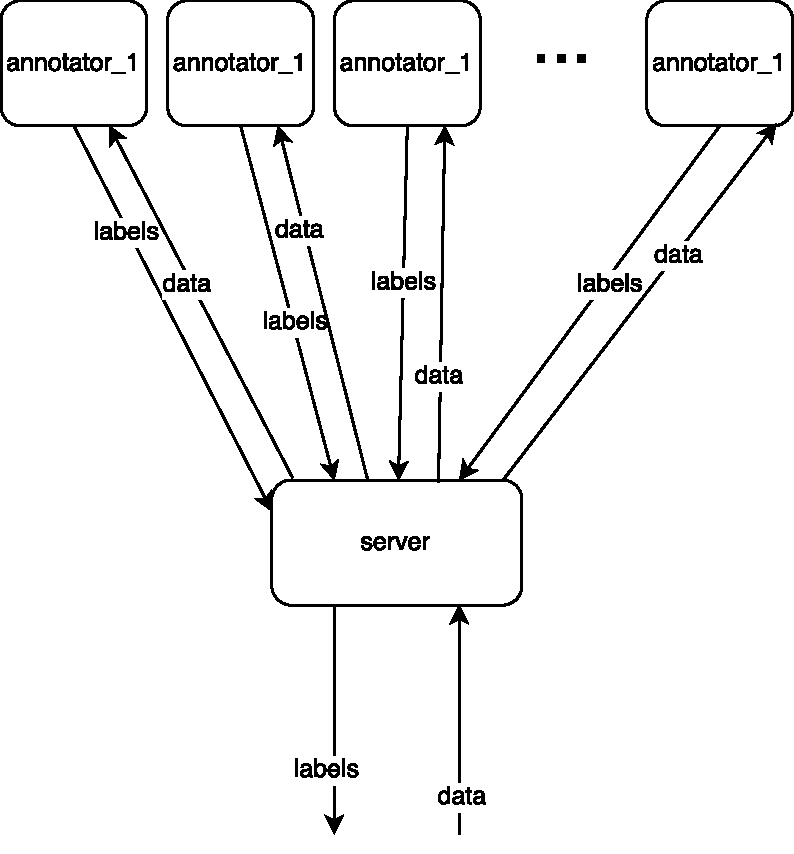
\includegraphics[width=0.5\textwidth]{figures/lowbudget.pdf}
  \label{fig:scheme}
\end{figure}

In training time, server forwards data to all the clients in order to retrieve annotations. Using the data annotated from a large set of clients, server trains a machine learning model that jointly learns the expertise of all the clients while minimizing the quadratic loss with respect to the ground truth.  

We design a method that would enable us to manage the tradeoff between model accuracy and communication effort. Furthermore, we impose a requirement that our methodology needs to be simple and compatible with a wide range of machine learning methods. 

Based on these requirements, our optimization model has a cost function consisting of three parts:

\begin{enumerate}
\item minimizing the error with respect to the ground truth
\item minimizing the error with respect ot the client annotations
\item making the client weight vector sparse 
\end{enumerate}

For example, the cost function for logistic regression looks like the following:

$$ L(w,v)= -\frac{1}{N} \sum_{n=1}^N (y_n \log \sum_{i=1}^M v_i\hat{y}_{ni} + (1-y_n) \log(1-\sum_{i=1}^M v_i \hat{y}_{ni})) + \psi \sum_{i=1}^{M} (y_{ni} - z_{ni})^2+\lambda \mid v \mid$$

$$ \sum_{i=1}^{M} v_i = 1 $$

where $y_n$ are ground truth labels for all training samples, $\hat{y}_{ni}$ are labels retrieved by querying  current client models, $z_{ni}$ are training labels from annotator clients, $v_i$ is a normalized vector of weights for all the clients.  

We want to use $L_1$ regularization to minimize the client weight vector. This is similar to the \textit{Lasso} feature selection, except that we select clients instead of features. 

The gradient is defined with the following equations:

$$ \frac{\partial L}{\partial w_j} = -\frac{1}{N} \sum_{n=1}^N (y_n \frac{1}{\sum_{i=1}^M v_i \hat{y}_{ni}} v_j \frac{\partial y_n}{\partial w_j} + (1-y_n) \frac{1}{1-\sum_{i=1}^M } v_j \frac{\partial y_n}{\partial w_j} + \psi \sum_{i=1}^M 2 (y_{ni} - z_{ni} \frac{\partial y_n}{\partial w_j}  ))$$

$$ \frac{\partial L}{\partial v_i} =  -\frac{1}{N} \sum_{n=1}^N (y_n \frac{1}{\sum_{i=1}^M v_i y_{ni}} + (1-\hat{y_n}) \frac{1} {1-\sum_{i=1}^M v_i y_{ni}} (-y_n) $$

The expression for the gradient $ \frac{y_n}{w_j}$ depends on the concrete method used to model the annotators.

 


For logistic regression we directly define the cost for the errors with respect to ground truth as crossentropy. However, with minimal changes our framework can also be usable with other machine learning methods. For example, we tested our methodology with neural networks as well. These methods, however, need to be convex or have a convex relaxation in order to still make a gradient-based optimization procedure work well.

In order to still use gradient descent as a convex optimization method with the $L_1$ norm, we use the method of subgradient when updating the value of $v$. The update that we derived is the following:

$$ v= v + S_{\lambda} (x-t_s \frac{y_n}{v}, \lambda)$$

where
$$ S_{\lambda} = 
\left\{
	\begin{array}{ll}
		x-\lambda  & \mbox{if } x > \lambda  \\
		x+\lambda & \mbox{if } x < -\lambda \\
		0 & \mbox{otherwise}
	\end{array}
\right.
$$

Furthermore, we normalize the values in the vector $v$ in order to retrieve the proper values of client weights:

$$ v = \frac{v}{\sum_{i=1}^M v_i} $$


 

\section{Results}

\section{Discussion}


\section{Conclusion}






% ---- Bibliography ----
%
\bibliographystyle{plain}
\bibliography{draft} % use this
%\clearpage
%\addtocmark[2]{Author Index} % additional numbered TOC entry
%\renewcommand{\indexname}{Author Index}
%\printindex
%\clearpage
%\addtocmark[2]{Subject Index} % additional numbered TOC entry
%\markboth{Subject Index}{Subject Index}
%\renewcommand{\indexname}{Subject Index}
%\input{subjidx.ind}
\end{document}
